\documentclass[11pt,a4paper]{article}
\usepackage[dvipsnames]{xcolor}
\usepackage{amsmath,tabularx,geometry,graphicx,multirow,tikz,listings,xfrac}

\usetikzlibrary{positioning}
\newdimen\nodeDist
\nodeDist=35mm
\geometry{a4paper, left=20mm, top=20mm}
\graphicspath{{../imgs/}}
\renewcommand\tabularxcolumn[1]{m{#1}}

\title{Aprendizagem 2021/22 Homework II - Group 66}
\author{João Cardoso, 99251. José João Ferreira, 99259}

\begin{document}

\color{darkgray}
\hspace{-8.25mm}
\begin{tabularx}{1.09\textwidth} {>{\raggedright\arraybackslash}X >{\centering\arraybackslash}X >{\raggedleft\arraybackslash}X}
  
\includegraphics[scale=0.2]{tecnico.pdf} &
  \textbf{Aprendizagem 2022/23} \par \textbf{Homework II - Group 66} &
  João Cardoso, 99251 \par José João Ferreira, 99259
\end{tabularx}
\color{black}

\begin{center}
\textbf{I. Pen-and-paper}
\end{center}

% PROBLEM 1
\begin{flushleft}
\textbf{1)}
\small
$ d(x_a, x_b) = Hamming(x_a, x_b) + \frac{1}{2} $ \hspace{7.5mm} $ kNN, \underline{k = 5} $ \par
\begin{tabularx}{1.09\textwidth}{X >{\hsize=.15\hsize}X X}
  \begin{center}
    \fbox{$ x_1 $}
  \end{center}
  $ d(x_1, x_2) = 1 + 1 + 0.5 = 2.5 $ \par
  $ d(x_1, x_3) = 0 + 1 + 0.5 = \textcolor{ForestGreen}{1.5} $ \hspace{3mm} $ x_3: z_3 = P $ \par
  $ d(x_1, x_4) = 0 + 0 + 0.5 = \textcolor{ForestGreen}{0.5} $ \hspace{3mm} $ x_4: z_4 = P $ \par
  $ d(x_1, x_5) = 1 + 0 + 0.5 = \textcolor{ForestGreen}{1.5} $ \hspace{3mm} $ x_5: z_5 = N $ \par
  $ d(x_1, x_6) = 1 + 0 + 0.5 = \textcolor{ForestGreen}{1.5} $ \hspace{3mm} $ x_6: z_6 = N $ \par
  $ d(x_1, x_7) = 0 + 1 + 0.5 = \textcolor{ForestGreen}{1.5} $ \hspace{3mm} $ x_7: z_7 = N $ \par
  $ d(x_1, x_8) = 1 + 1 + 0.5 = 2.5 $ \par
  \vspace{3mm} $ \hat{z_1} = w\_mode((\frac{1}{1.5}+\frac{1}{0.5})P, (\frac{1}{1.5}+\frac{1}{1.5}+\frac{1}{1.5})N) $ \par
  \vspace{1mm}\hspace{3mm} $ = w\_mode(\frac{8}{3}P, 2N) = N $
  & &
  \begin{center}
    \fbox{$ x_2 $}
  \end{center}
  $ d(x_2, x_1) = 2.5 $ \par
  $ d(x_2, x_3) = 1 + 0 + 0.5 = \textcolor{ForestGreen}{1.5} $ \hspace{3mm} $ x_3: z_3 = P $ \par
  $ d(x_2, x_4) = 1 + 1 + 0.5 = 2.5 $ \par
  $ d(x_2, x_5) = 0 + 1 + 0.5 = \textcolor{ForestGreen}{1.5} $ \hspace{3mm} $ x_5: z_5 = N $ \par
  $ d(x_2, x_6) = 0 + 1 + 0.5 = \textcolor{ForestGreen}{1.5} $ \hspace{3mm} $ x_6: z_6 = N $ \par
  $ d(x_2, x_7) = 1 + 0 + 0.5 = \textcolor{ForestGreen}{1.5} $ \hspace{3mm} $ x_7: z_7 = N $ \par
  $ d(x_2, x_8) = 0 + 0 + 0.5 = \textcolor{ForestGreen}{0.5} $ \hspace{3mm} $ x_8: z_8 = N $ \par
  \vspace{3mm} $ \hat{z_2} = w\_mode((\frac{1}{1.5})P, (\frac{1}{1.5}+\frac{1}{1.5}+\frac{1}{1.5}+\frac{1}{0.5})N) $ \par
  \vspace{1mm}\hspace{3mm} $ = w\_mode(\frac{2}{3}P, 4N) = N $
\end{tabularx}
\begin{tabularx}{1.09\textwidth}{X >{\hsize=.25\hsize}X X >{\hsize=.25\hsize}X X}
  \begin{center}
    \fbox{$ x_3 $}
  \end{center}
  $ d(x_3, x_1) = \textcolor{ForestGreen}{1.5} $ \hspace{3mm} $ z_1 = P $ \par
  $ d(x_3, x_2) = \textcolor{ForestGreen}{1.5} $ \hspace{3mm} $ z_2 = P $ \par
  $ d(x_3, x_4) = \textcolor{ForestGreen}{1.5} $ \hspace{3mm} $ z_4 = P $ \par
  $ d(x_3, x_5) = 2.5 $ \par
  $ d(x_3, x_6) = 2.5 $ \par
  $ d(x_3, x_7) = \textcolor{ForestGreen}{0.5} $ \hspace{3mm} $ z_7 = N $ \par
  $ d(x_3, x_8) = \textcolor{ForestGreen}{1.5} $ \hspace{3mm} $ z_8 = N $ \par
  \vspace{3mm} $ \hat{z_3} = wm(2P, \frac{8}{3}N) = N $
  & &
  \begin{center}
    \fbox{$ x_4 $}
  \end{center}
  $ d(x_4, x_1) = \textcolor{ForestGreen}{0.5} $ \hspace{3mm} $ z_1 = P $ \par
  $ d(x_4, x_2) = 2.5 $ \par
  $ d(x_4, x_3) = \textcolor{ForestGreen}{1.5} $ \hspace{3mm} $ z_3 = P $ \par
  $ d(x_4, x_5) = \textcolor{ForestGreen}{1.5} $ \hspace{3mm} $ z_5 = N $ \par
  $ d(x_4, x_6) = \textcolor{ForestGreen}{1.5} $ \hspace{3mm} $ z_6 = N $ \par
  $ d(x_4, x_7) = \textcolor{ForestGreen}{1.5} $ \hspace{3mm} $ z_7 = N $ \par
  $ d(x_4, x_8) = 2.5 $ \par
  \vspace{3mm} $ \hat{z_4} = wm(\frac{8}{3}P, 2N) = P $
  & &
  \begin{center}
    \fbox{$ x_5 $}
  \end{center}
  $ d(x_5, x_1) = \textcolor{ForestGreen}{1.5} $ \hspace{3mm} $ z_1 = P $ \par
  $ d(x_5, x_2) = \textcolor{ForestGreen}{1.5} $ \hspace{3mm} $ z_2 = P $ \par
  $ d(x_5, x_3) = 2.5 $ \par
  $ d(x_5, x_4) = \textcolor{ForestGreen}{1.5} $ \hspace{3mm} $ z_4 = P $ \par
  $ d(x_5, x_6) = \textcolor{ForestGreen}{0.5} $ \hspace{3mm} $ z_6 = N $ \par
  $ d(x_5, x_7) = 2.5 $ \par
  $ d(x_5, x_8) = \textcolor{ForestGreen}{1.5} $ \hspace{3mm} $ z_8 = N $ \par
  \vspace{3mm} $ \hat{z_5} = wm(2P, \frac{8}{3}N) = N $
\end{tabularx}
\begin{tabularx}{1.09\textwidth}{X >{\hsize=.25\hsize}X X >{\hsize=.25\hsize}X X}
  \begin{center}
    \fbox{$ x_6 $}
  \end{center}
  $ d(x_6, x_1) = \textcolor{ForestGreen}{1.5} $ \hspace{3mm} $ z_1 = P $ \par
  $ d(x_6, x_2) = \textcolor{ForestGreen}{1.5} $ \hspace{3mm} $ z_2 = P $ \par
  $ d(x_6, x_3) = 2.5 $ \par
  $ d(x_6, x_4) = \textcolor{ForestGreen}{1.5} $ \hspace{3mm} $ z_4 = P $ \par
  $ d(x_6, x_5) = \textcolor{ForestGreen}{0.5} $ \hspace{3mm} $ z_5 = N $ \par
  $ d(x_6, x_7) = 2.5 $ \par
  $ d(x_6, x_8) = \textcolor{ForestGreen}{1.5} $ \hspace{3mm} $ z_8 = N $ \par
  \vspace{3mm} $ \hat{z_6} = wm(2P, \frac{8}{3}N) = N $
  & &
  \begin{center}
    \fbox{$ x_7 $}
  \end{center}
  $ d(x_7, x_1) = \textcolor{ForestGreen}{1.5} $ \hspace{3mm} $ z_1 = P $ \par
  $ d(x_7, x_2) = \textcolor{ForestGreen}{1.5} $ \hspace{3mm} $ z_2 = P $ \par
  $ d(x_7, x_3) = \textcolor{ForestGreen}{0.5} $ \hspace{3mm} $ z_3 = P $ \par
  $ d(x_7, x_4) = \textcolor{ForestGreen}{1.5} $ \hspace{3mm} $ z_4 = P $ \par
  $ d(x_7, x_5) = 2.5 $ \par
  $ d(x_7, x_6) = 2.5 $ \par
  $ d(x_7, x_8) = \textcolor{ForestGreen}{1.5} $ \hspace{3mm} $ z_8 = N $ \par
  \vspace{3mm} $ \hat{z_7} = wm(4P, \frac{2}{3}N) = P $
  & &
  \begin{center}
    \fbox{$ x_8 $}
  \end{center}
  $ d(x_8, x_1) = 2.5 $ \par
  $ d(x_8, x_2) = \textcolor{ForestGreen}{0.5} $ \hspace{3mm} $ z_2 = P $ \par
  $ d(x_8, x_3) = \textcolor{ForestGreen}{1.5} $ \hspace{3mm} $ z_3 = P $ \par
  $ d(x_8, x_4) = 2.5 $ \par
  $ d(x_8, x_5) = \textcolor{ForestGreen}{1.5} $ \hspace{3mm} $ z_5 = N $ \par
  $ d(x_8, x_6) = \textcolor{ForestGreen}{1.5} $ \hspace{3mm} $ z_6 = N $ \par
  $ d(x_8, x_7) = \textcolor{ForestGreen}{1.5} $ \hspace{3mm} $ z_7 = N $ \par
  \vspace{3mm} $ \hat{z_8} = wm(\frac{8}{3}P, 2N) = P $
  \end{tabularx}

  \vspace{5mm}
  \begin{tabularx}{1.09\textwidth}{>{\hsize=.5\hsize}X X}
    \begin{tabular}{c|cc|c|c}
            & $y_1$ & $y_2$ & $z$ & $\hat{z}$ \\ \hline
      $x_1$ & A     & 0     & P   & P         \\
      $x_2$ & B     & 1     & P   & N         \\
      $x_3$ & A     & 1     & P   & N         \\
      $x_4$ & A     & 0     & P   & P         \\ \hline
      $x_5$ & B     & 0     & N   & N         \\
      $x_6$ & B     & 0     & N   & N         \\
      $x_7$ & A     & 1     & N   & P         \\
      $x_8$ & B     & 1     & N   & P        
    \end{tabular}
    &
    \vspace{10mm}\begin{tabular}{llcc}
                                                                 &                        & \multicolumn{2}{c}{$z$} \\
                                                                 & \multicolumn{1}{l|}{}  & \multicolumn{1}{c|}{P}   & N   \\ \cline{2-4} 
    \multicolumn{1}{c}{\multirow{2}{*}{$\hat{z}$}} & \multicolumn{1}{c|}{P} & \multicolumn{1}{c|}{2}   & 2   \\ \cline{2-4} 
    \multicolumn{1}{c}{}                                         & \multicolumn{1}{c|}{N} & \multicolumn{1}{c|}{2}   & 2
    \end{tabular} \par
    \vspace{5mm} $ Recall = \frac{TP}{TP + FN} = \frac{2}{2 + 2} = \frac{1}{2} $
  \end{tabularx}
\end{flushleft}
\normalsize

% PAGE BREAK
\pagebreak
\color{darkgray}
\hspace{-8.25mm}
\begin{tabularx}{1.09\textwidth} {>{\raggedright\arraybackslash}X >{\centering\arraybackslash}X >{\raggedleft\arraybackslash}X}
  
\includegraphics[scale=0.2]{tecnico.pdf} &
  \textbf{Aprendizagem 2022/23} \par \textbf{Homework II - Group 66} &
  João Cardoso, 99251 \par José João Ferreira, 99259
\end{tabularx}
\color{black}

\begin{center}
  \textbf{ }
\end{center}

% PROBLEM 2
\begin{flushleft}
\textbf{2)}
\small
\vspace{-3mm}\begin{flalign*}
  P(class = c|x_{new}) &= \frac{P(x = x_{new} | class = c) \cdot P(class = c)}{P(x = x_{new})} &&\\
  &= \frac{P(y_1 = y_{1\_new}, y_2 = y_{2\_new} | class = c) \cdot P(y_3 = y_{3\_new} | class = c) \cdot P(class = c)}{P(y_1 = y_{1\_new}, y_2 = y_{2\_new}) \cdot P(y_3 = y_{3\_new})} &&\\
\end{flalign*}

Priors:\hspace{5mm}$ P(class = P) = \frac{5}{9} $ \hspace{5mm} $ P(class = N) = \frac{4}{9} $ \par
\vspace{5mm}
\begin{tabularx}{1.09\textwidth}{>{\hsize=.9\hsize}X X}
  \fbox{$ P(y_1 = y_{1\_new}, y_2 = y_{2\_new} | class = c) $} \par
  \vspace{2.5mm}\begin{tabular}{cccc}
    $y_1$ & $y_2$ & $c$ & $P(y_1,y_2|class = c$) \\ \hline
    A     & 0     & P   & $\sfrac{2}{5}$         \\ \hline
    A     & 1     & P   & $\sfrac{1}{5}$         \\ \hline
    B     & 0     & P   & $\sfrac{1}{5}$         \\ \hline
    B     & 1     & P   & $\sfrac{1}{5}$         \\ \hline
    A     & 0     & N   & $0$                    \\ \hline
    A     & 1     & N   & $\sfrac{1}{4}$         \\ \hline
    B     & 0     & N   & $\sfrac{2}{4}$         \\ \hline
    B     & 1     & N   & $\sfrac{1}{4}$        
  \end{tabular}
  &
  \fbox{$ P(y_1 = y_{1\_new}, y_2 = y_{2\_new}) $} \par
  \vspace{2.5mm}\begin{tabular}{ccc}
    $y_1$ & $y_2$ & $P(y_1,y_2)$   \\ \hline
    A     & 0     & $\sfrac{2}{9}$ \\ \hline
    A     & 1     & $\sfrac{2}{9}$ \\ \hline
    B     & 0     & $\sfrac{3}{9}$ \\ \hline
    B     & 1     & $\sfrac{2}{9}$ \\
  \end{tabular}
\end{tabularx}

\vspace{5mm} \fbox{$ P(y_3 = y_{3\_new} | class = P) $}
\begin{flalign*}
&v = y_3|P = \{1.2, 0.8, 0.5, 0.9, 0.8\} &&\\
&\mu = \frac{\sum(y_{3\_i})}{size(v)} = 0.84 &&\\
&\sigma^2 = \frac{\sum(y_{3\_i} - \mu)^2}{size(v) - 1} = 0.063 &&\\
&P(y_3 = y_{3\_new} | class = P) = \underline{N(y_{3\_new} | \mu = 0.84, \sigma^2 = 0.063)} &&\\
\end{flalign*}

\fbox{$ P(y_3 = y_{3\_new} | class = N) $}
\begin{flalign*}
&v = y_3|N = \{1, 0.9, 1.2, 0.8\} &&\\
&\mu = 0.975 &&\\
&\sigma^2 \approx 0.029 &&\\
&P(y_3 = y_{3\_new} | class = N) = \underline{N(y_{3\_new} | \mu = 0.975, \sigma^2 = 0.029)} &&\\
\end{flalign*}

\fbox{$ P(y_3 = y_{3\_new}) $}
\begin{flalign*}
&val = \{1.2, 0.8, 0.5, 0.9, 0.8, 1, 0.9, 1.2, 0.8\} &&\\
&\mu = 0.9 &&\\
&\sigma^2 = 0.0475 &&\\
&P(y_3 = y_{3\_new}) = \underline{N(y_{3\_new} | \mu = 0.9, \sigma^2 = 0.0475)} &&\\
\end{flalign*}
\end{flushleft}
\normalsize

% PAGE BREAK
\pagebreak
\color{darkgray}
\hspace{-8.25mm}
\begin{tabularx}{1.09\textwidth} {>{\raggedright\arraybackslash}X >{\centering\arraybackslash}X >{\raggedleft\arraybackslash}X}
  
\includegraphics[scale=0.2]{tecnico.pdf} &
  \textbf{Aprendizagem 2022/23} \par \textbf{Homework II - Group 66} &
  João Cardoso, 99251 \par José João Ferreira, 99259
\end{tabularx}
\color{black}

\begin{center}
  \textbf{ }
\end{center}

% PROBLEM 3
\begin{flushleft}
\textbf{3)} \par
\small

\begin{tabularx}{1.09\textwidth}{>{\hsize=.9\hsize}X X}
  \vspace{1mm}\begin{tabular}{c|c|c|c|c|}
    \cline{2-5}
                                  & $y_1$ & $y_2$ & $y_3$ & $class$ \\ \hline
    \multicolumn{1}{|c|}{$x_{t1}$} & A     & 1     & 0.8   & P       \\ \hline
  \end{tabular}
  &
  $ h_{MAP} = argmax_{h \in H}P(h|D) $
\end{tabularx} \par
  \vspace{3.5mm}\small $ P(class = P | x_{t1}) = \frac{P(x_{t1} | class = P) \cdot P(class = P)}{P(x_{t1} | class = P) \cdot P(class = P) + P(x_{t1} | class = N) \cdot P(class = N)} $ \par
  \vspace{2mm}\footnotesize $ = \frac{P(y_1 = A, y_2 = 1 | class = P) \cdot P(y_3 = 0.8 | class = P) \cdot P(class = P)}{P(y_1 = A, y_2 = 1 | class = P) \cdot P(y_3 = 0.8 | class = P) \cdot P(class = P) + P(y_1 = A, y_2 = 1 | class = N) \cdot P(y_3 = 0.8 | class = N) \cdot P(class = N)} $ \par
  \vspace{2mm}\footnotesize $ = \frac{P(y_1 = A, y_2 = 1 | class = P) \cdot N(y_3 = 0.8 | \mu = 0.84, \sigma^2 = 0.063) \cdot P(class = P)}{P(y_1 = A, y_2 = 1 | class = P) \cdot N(y_3 = 0.8 | \mu = 0.84, \sigma^2 = 0.063) \cdot P(class = P) + P(y_1 = A, y_2 = 1 | class = N) \cdot N(y_3 = 0.8 | \mu = 0.975, \sigma^2 = 0.029) \cdot P(class = N)} $ \par
  \vspace{2mm}\small $ = \frac{\sfrac{1}{5} \times 1.569369 \times \sfrac{5}{9}}{\sfrac{1}{5} \times 1.569369 \times \sfrac{5}{9} + \sfrac{1}{4} \times 1.381643 \times \sfrac{4}{9}} $ \par
  \vspace{2.5mm}\small $ \approx 0.5318 $ \par

\vspace{6mm}\begin{tabular}{c|c|c|c|c|}
  \cline{2-5}
                                 & $y_1$ & $y_2$ & $y_3$ & $class$ \\ \hline
  \multicolumn{1}{|c|}{$x_{t2}$} & B     & 1     & 1     & P       \\ \hline
\end{tabular} \par
  \vspace{3.5mm}\small $ P(class = P | x_{t2}) = \frac{P(x_{t2} | class = P) \cdot P(class = P)}{P(x_{t2} | class = P) \cdot P(class = P) + P(x_{t2} | class = N) \cdot P(class = N)} $ \par
  \vspace{2mm}\footnotesize $ = \frac{P(y_1 = B, y_2 = 1 | class = P) \cdot P(y_3 = 1 | class = P) \cdot P(class = P)}{{P(y_1 = B, y_2 = 1 | class = P) \cdot P(y_3 = 1 | class = P) \cdot P(class = P) + P(y_1 = B, y_2 = 1 | class = N) \cdot P(y_3 = 1 | class = N) \cdot P(class = N)}} $ \par
  \vspace{2mm}\footnotesize $ = \frac{P(y_1 = B, y_2 = 1 | class = P) \cdot N(y_3 = 1 | \mu = 0.84, \sigma^2 = 0.063) \cdot P(class = P)}{P(y_1 = B, y_2 = 1 | class = P) \cdot N(y_3 = 1 | \mu = 0.84, \sigma^2 = 0.063) \cdot P(class = P) + P(y_1 = B, y_2 = 1 | class = N) \cdot N(y_3 = 1 | \mu = 0.975, \sigma^2 = 0.029) \cdot P(class = N)} $ \par
  \vspace{2mm}\small $ = \frac{\sfrac{1}{5} \times 1.297186 \times \sfrac{5}{9}}{\sfrac{1}{5} \times 1.297186 \times \sfrac{5}{9} + \sfrac{1}{4} \times 2.317560976003106 \times \sfrac{4}{9}} $ \par
  \vspace{2.5mm}\small $ \approx 0.3588 $ \par

\vspace{6mm}\begin{tabular}{c|c|c|c|c|}
  \cline{2-5}
                                 & $y_1$ & $y_2$ & $y_3$ & $class$ \\ \hline
  \multicolumn{1}{|c|}{$x_{t3}$} & B     & 0     & 0.9   & N       \\ \hline
  \end{tabular} \par
  \vspace{3.5mm}\small $ P(class = P | x_{t3}) = \frac{P(x_{t3} | class = P) \cdot P(class = P)}{P(x_{t3} | class = P) \cdot P(class = P) + P(x_{t3} | class = N) \cdot P(class = N)} $ \par
  \vspace{2mm}\footnotesize $ = \frac{P(y_1 = B, y_2 = 0 | class = P) \cdot P(y_3 = 0.9 | class = P) \cdot P(class = P)}{{P(y_1 = B, y_2 = 0 | class = P) \cdot P(y_3 = 0.9 | class = P) \cdot P(class = P) + P(y_1 = B, y_2 = 0 | class = N) \cdot P(y_3 = 0.9 | class = N) \cdot P(class = N)}} $ \par
  \vspace{2mm}\footnotesize $ = \frac{P(y_1 = B, y_2 = 0 | class = P) \cdot N(y_3 = 0.9 | \mu = 0.84, \sigma^2 = 0.063) \cdot P(class = P)}{P(y_1 = B, y_2 = 0 | class = P) \cdot N(y_3 = 0.9 | \mu = 0.84, \sigma^2 = 0.063) \cdot P(class = P) + P(y_1 = B, y_2 = 0 | class = N) \cdot N(y_3 = 0.9 | \mu = 0.975, \sigma^2 = 0.029) \cdot P(class = N)} $ \par
  \vspace{2mm}\small $ = \frac{\sfrac{1}{5} \times 1.544655 \times \sfrac{5}{9}}{\sfrac{1}{5} \times 1.544655 \times \sfrac{5}{9} + \sfrac{2}{4} \times 2.126140645404257 \times \sfrac{4}{9}} $ \par
  \vspace{2.5mm}\small $ \approx 0.2664 $ \par
\end{flushleft}
\normalsize

% PROBLEM 4
\begin{flushleft}\vspace{2mm}
\textbf{4)}
The decision threshold that optimizes testing accuracy is $\theta = 0.3$, seeing as it is the only one where observation $x_{t3}$ is classified as negative, while observations $x_{t1}$ and $x_{t2}$ are classified as positive, meaning that both positives are true positives and the negative is a true negative. With a threshold value of 0.5, all but one observation would be classified as negative, resulting in one false negative, and with a value of 0.7, all the observations would be classified as negative, resulting in two false negatives. As such, the accuracy value is $\sfrac{3}{3} = 1$ for $\theta = 0.3$, $\sfrac{2}{3}$ for $\theta = 0.5$ and $\sfrac{1}{3}$ for $\theta = 0.7$.
\end{flushleft}

\pagebreak

\color{darkgray}
\hspace{-8.25mm}
\begin{tabularx}{1.09\textwidth} {>{\raggedright\arraybackslash}X >{\centering\arraybackslash}X >{\raggedleft\arraybackslash}X}
  
\includegraphics[scale=0.2]{tecnico.pdf} &
  \textbf{Aprendizagem 2022/23} \par \textbf{Homework II - Group 66} &
  João Cardoso, 99251 \par José João Ferreira, 99259
\end{tabularx}
\color{black}

\begin{center}
\textbf{II. Programming and critical analysis}
\end{center}

% PROBLEM 5
\begin{flushleft}
\textbf{5)} \par
\begin{center}
\vspace{-4.5mm}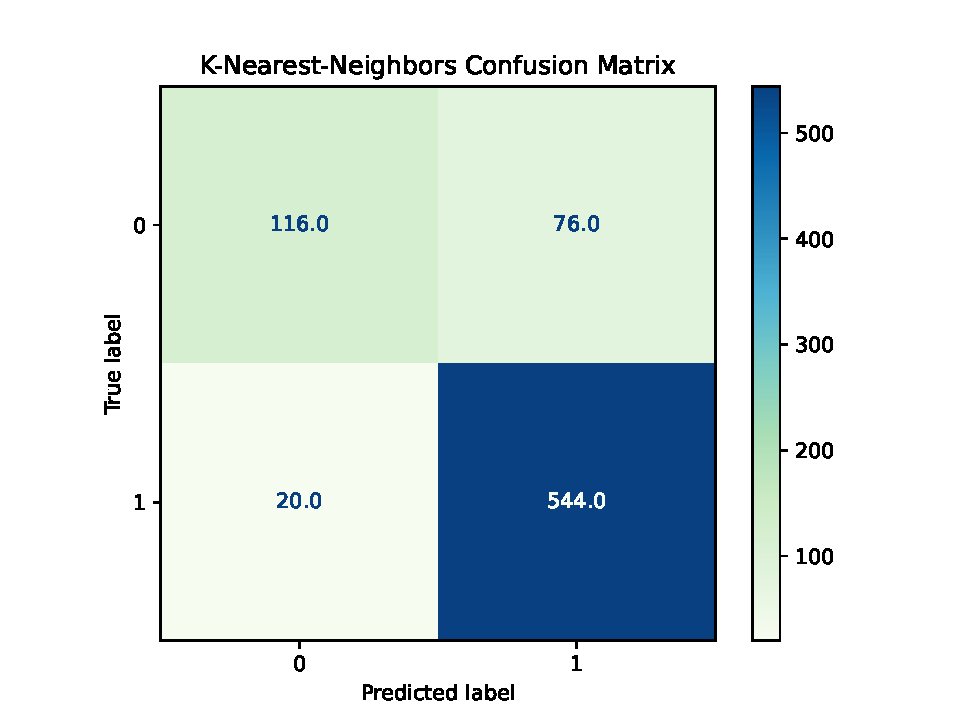
\includegraphics[scale=0.8]{hw02_plot_knn.pdf}
\vspace{8.5mm}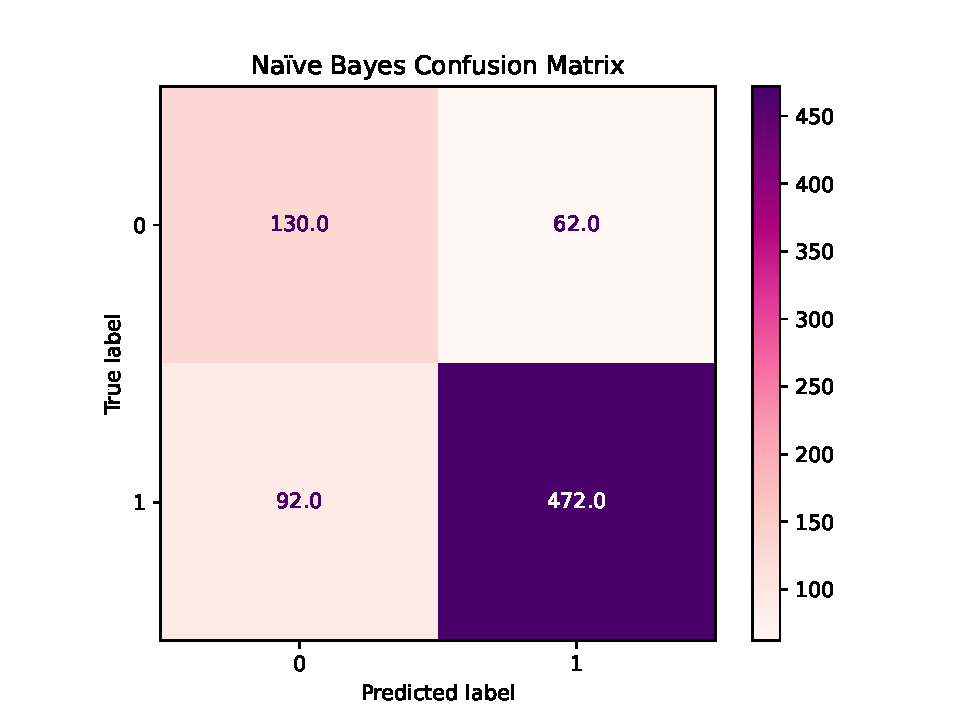
\includegraphics[scale=0.8]{hw02_plot_nb.pdf}
\end{center}
\end{flushleft}
\vspace*{2mm}

\pagebreak

\color{darkgray}
\hspace{-8.25mm}
\begin{tabularx}{1.09\textwidth} {>{\raggedright\arraybackslash}X >{\centering\arraybackslash}X >{\raggedleft\arraybackslash}X}
  
\includegraphics[scale=0.2]{tecnico.pdf} &
  \textbf{Aprendizagem 2022/23} \par \textbf{Homework II - Group 66} &
  João Cardoso, 99251 \par José João Ferreira, 99259
\end{tabularx}
\color{black}

\begin{center}
\textbf{ }
\end{center}

% PROBLEM 6
\begin{flushleft}
\textbf{6)}
  The statement is true. If we calculate the p-value of the t-test in a paired setting, as is the case here (estimates of the same size), between the $kNN$ predictor and the Naïve Bayes predictor, for the hypothesis "$kNN > NB$", the result is approximately $0.001317$. Thus, we observe that the performance of the $kNN$ predictor is better than the $NB$ predictor with statistical significance below a confidence level of $0.05$, since $0.001317 < 0.05$.
  \par
  In fact, a simple analysis of the confusion matrices would be enough to realize that $kNN$ is a classifier with greater prediction accuracy. If we add the true positives to the true negatives in both matrices presented above, which corresponds to the value of correctly classified observations in relation to the real value, we conclude that the kNN has a higher value, therefore, it is more precise.
\end{flushleft}

% PROBLEM 7
\vspace{2.5mm}
\begin{flushleft}
\textbf{7)}
  k-Nearest-Neighbors yields greater predictive accuracy than Naïve Bayes, according to our measurements. We speculate that this may be due to three reasons. The first one is that the value for $k$ in $kNN$ is sufficiently large to achieve a tight fit to the data. Additionally, since the data were normalized, $kNN$ was better suited as a classifier. Lastly, seeing as Naïve Bayes is a linear classifier, we suspect that the data might not have been linearly separate to enough of an extent to enable Naïve Bayes to outperform $kNN$ accuracy-wise.
\end{flushleft}

\pagebreak

\color{darkgray}
\hspace{-8.25mm}
\begin{tabularx}{1.09\textwidth} {>{\raggedright\arraybackslash}X >{\centering\arraybackslash}X >{\raggedleft\arraybackslash}X}
  
\includegraphics[scale=0.2]{tecnico.pdf} &
  \textbf{Aprendizagem 2022/23} \par \textbf{Homework II - Group 66} &
  João Cardoso, 99251 \par José João Ferreira, 99259
\end{tabularx}
\color{black}

\begin{center}
\textbf{III. Appendix}
\end{center}

\definecolor{backcolour}{rgb}{0.95,0.95,0.92}
\definecolor{codegreen}{rgb}{0,0.6,0}
\definecolor{codepurple}{rgb}{0.58,0,0.82}
\definecolor{codegray}{rgb}{0.5,0.5,0.5}
\definecolor{codered}{rgb}{0.75,0.25,0}
\definecolor{codeyellow}{rgb}{0.55,0.55,0.0}
\definecolor{codeForestGreen}{rgb}{0.05,0.65,0.55}

\lstdefinestyle{mystyle}{
    backgroundcolor=\color{backcolour},
    commentstyle=\color{codegreen},
    keywordstyle=\color{codepurple},
    numberstyle=\tiny\color{codegray},
    stringstyle=\color{codered},
    emph=[0]{loadarff,confusion_matrix,accuracy_score,ttest_rel,drop,fit_transform,zeros,split,fit,predict,append,plot,set_title,print},
    emphstyle=[0]\color{codeyellow},
    emph=[1]{scipy,io,arff,pandas,pd,DataFrame,sklearn,preprocessing,numpy,np,LabelEncoder,StandardScaler,model_selection,StratifiedKFold,neighbors,KNeighborsClassifier,naive_bayes,GaussianNB,metrics,ConfusionMatrixDisplay,stats},
    emphstyle=[1]\color{codeForestGreen},
    basicstyle=\ttfamily\footnotesize,
    breakatwhitespace=false,
    breaklines=true,
    captionpos=b,
    keepspaces=true,
    numbers=left,
    numbersep=7.5pt,
    showspaces=false,
    showstringspaces=false,
    showtabs=false,
    tabsize=2,
    language=Python,
    morekeywords={as}}
\lstset{style=mystyle}

\hspace{-8.25mm}
\begin{tabularx}{1.09\textwidth}{X}
  \lstinputlisting{hw02.py}
\end{tabularx}

\end{document}